% !TEX program = xelatex
% !TEX encoding = UTF-8 Unicode
\documentclass{beamer}
\usepackage[no-math]{fontspec}
\usepackage{xeCJK}
\hypersetup{colorlinks,linkcolor=}

\usetheme{CambridgeUS}
\title{Bit-true arithmetics}
\author[jdh8]{何震邦 (Chen-Pang He, jdh8)}
\date{March 19, 2025}
\institute{Skymizer}

\begin{document}
\maketitle

\section{Overview}
\begin{frame}{Overview}
	\tableofcontents
\end{frame}

\begin{frame}{Why}
	\begin{block}{\Huge``}
		\vspace{-1em}
		\begin{enumerate}
			\item The need for an unambiguous specification of the most frequent functions
			\item The only specification that makes sense is correct rounding
			\item Now, correct rounding of many functions is feasible at a very reasonable cost
		\end{enumerate}

		--- Nicolas Brisebarre, Guillaume Hanrot, Jean-Michel Muller, Paul Zimmermann.
		\href
		{https://hal.science/hal-04474530/document}
		{Correctly-rounded evaluation of a function: why, how, and at what cost?}
		2025.  hal-04474530v3
	\end{block}
\end{frame}

\begin{frame}{Quantization}
	\begin{itemize}
		\item Quantization maps a large/continuous set to a small/countable set.
		\item Quantization is required because we only have finite bits to store data.
		\item Further quantization reduces space and probably time usage.
	\end{itemize}
\end{frame}

\begin{frame}{Accuracy and precision}
	\begin{figure}
		\caption{
			\href
			{https://en.wikipedia.org/wiki/Accuracy_and_precision\#ISO_definition_(ISO_5725)}
			{Accuracy according to BIPM and ISO 5725}
		}
		\begin{minipage}{0.4\textwidth}
			\centering
			\href
			{https://upload.wikimedia.org/wikipedia/commons/1/10/High_accuracy_Low_precision.svg}
			{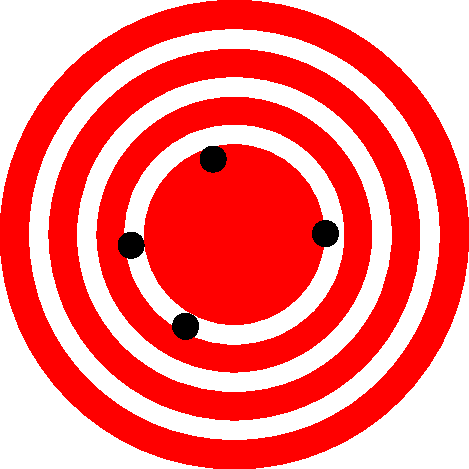
\includegraphics[width=0.8\textwidth]{assets/High_accuracy_Low_precision.pdf}} \\
			Low accuracy due to low precision
		\end{minipage}
		\begin{minipage}{0.4\textwidth}
			\centering
			\href
			{https://upload.wikimedia.org/wikipedia/commons/3/3a/High_precision_Low_accuracy.svg}
			{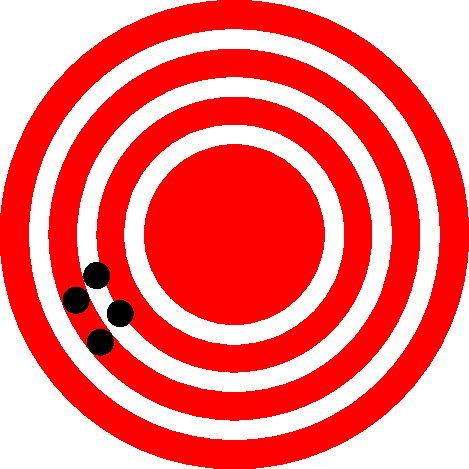
\includegraphics[width=0.8\textwidth]{assets/High_precision_Low_accuracy.pdf}} \\
			Low accuracy despite of high precision
		\end{minipage}
	\end{figure}
\end{frame}

\begin{frame}{Rounding modes}
	\begin{figure}
		\href
		{https://upload.wikimedia.org/wikipedia/commons/8/8a/Comparison_rounding_graphs_SMIL.svg}
		{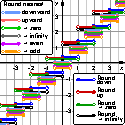
\includegraphics[height=0.625\textheight]{assets/Comparison_rounding_graphs_SMIL.pdf}}

		\caption{
			\href{https://upload.wikimedia.org/wikipedia/commons/8/8a/Comparison_rounding_graphs_SMIL.svg}{Interactive graph}
			by CMG Lee on
			\href{https://commons.wikimedia.org/wiki/File:Comparison_rounding_graphs_SMIL.svg}{Wikimedia Commons}
		}
	\end{figure}
\end{frame}

\section{Algebraic functions}
\subsection{Floating-point format}
\begin{frame}{IEEE 754 binary formats}
	\begin{example}
		\begin{figure}
			\href
			{https://upload.wikimedia.org/wikipedia/commons/d/d2/Float_example.svg}
			{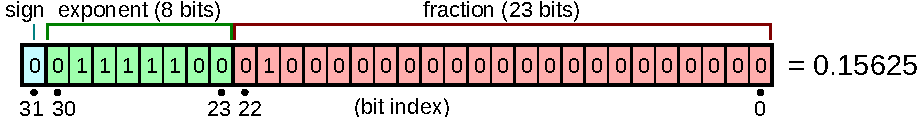
\includegraphics[width=0.8\textwidth]{assets/Float_example.pdf}}
			\[ 1.{\color{red}01}_2 \times 2^{{\color{green}124} - 127}  \]
			\begin{center}
				\ttfamily 0x1.{\color{red}4}p{\color{green}-3}
			\end{center}
			\caption{Example normal binary32 by
				\href{https://en.wikipedia.org/wiki/User:Fresheneesz}{Fresheneesz} on
				\href{https://commons.wikimedia.org/wiki/File:Float_example.svg}{English Wikipedia}
			}
		\end{figure}
		\begin{itemize}
			\item (Exponent) bias defaults to $2^{E-1} - 1$.
			\item Implicit bit (1) leads the significand/mantissa.
		\end{itemize}
	\end{example}
\end{frame}

\begin{frame}{Floating-point classification}
	\[
		\begin{cases}
			\text{Infinity | NaN},   & \text{if exponent} = 2^E - 1 \\
			\text{Subnormal | zero}, & \text{if exponent} = 0       \\
			\text{Normal},           & \text{otherwise}
		\end{cases}
	\]
\end{frame}

\begin{frame}{Subnormal numbers}
	When the stored exponent is 0,
	\begin{itemize}
		\item The exponent is deemed as 1.
		\item Instead, the implicit bit becomes 0.
	\end{itemize}

	\begin{figure}
		\href
		{https://upload.wikimedia.org/wikipedia/commons/6/69/Denormalized_numbers_on_a_line.svg}
		{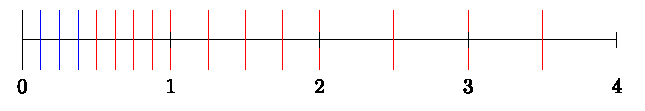
\includegraphics[width=0.8\textwidth]{assets/Denormalized_numbers_on_a_line.pdf}}

		\caption{Seamless transition from 0 to normal numbers by
			\href{https://en.wikipedia.org/wiki/User:Blacklemon67}{Blacklemon67} on
			\href{https://commons.wikimedia.org/wiki/File:Denormalized_numbers_on_a_line.svg}{English Wikipedia}
		}
	\end{figure}
\end{frame}

\begin{frame}{Quiz}
	What is \texttt{std::bit\_cast<float>(0x40000000)}?
\end{frame}

\subsection{Rounding}
\begin{frame}{Arithmetics}
	Arithmetic results can be inexact in the target format.

	\begin{example}
		Consider 0.1 + 0.2 in IEEE 754 binary64 format.

		\begin{itemize}
			\item 0.1 $\approx$ \texttt{0x1.999999999999ap-4} = \texttt{0x0.6666666666666{\color{red}4}p-2}
			\item 0.2 $\approx$ \texttt{0x1.999999999999ap-3} = \texttt{0x0.ccccccccccccc{\color{red}8}p-2}
			\item 0.3 $\approx$ \texttt{0x1.3333333333333p-2}
		\end{itemize}
		\begin{align*}
			 & \text{binary64}(0.1) + \text{binary64}(0.2)
			\\ ={}& \texttt{0x1.3333333333333{\color{red}c}p-2}
			\\ \approx{}& \texttt{0x1.3333333333334p-2}
			\\ \approx{}& 0.30000000000000004
		\end{align*}
	\end{example}
\end{frame}

\begin{frame}{Double rounding problem}
	\begin{itemize}
		\item Rounding is not associative!
		\item 9.46 $\to$ 9
		\item 9.46 $\to$ 9.5 $\to$ 10
	\end{itemize}
\end{frame}

\begin{frame}{\href
		{https://hal-lara.archives-ouvertes.fr/hal-02101979/document}
		{When double rounding is odd}
	}
	\begin{block}{Odd rounding}
		\[
			\operatorname\square_{\text{odd}} x =
			\begin{cases}
				x,                               & \text{if } x \text{ has exact representation}            \\
				\operatorname\bigtriangleup x,   & \textup{if} \operatorname\bigtriangleup x \text{ is odd} \\
				\operatorname\bigtriangledown x, & \text{otherwise}
			\end{cases}
		\]
	\end{block}

	\begin{block}{Correct double rounding algorithm}
		Given a binary format with precision of $p$ bits and an extended binary
		format of $p + k$ bits,
		\[
			\operatorname\circ^p \operatorname\square_{\textup{odd}}^{p + k} x = \operatorname\circ^p x
		\]
		when $p \ge 2$, $k \ge 2$, and the result does not over- or underflow.
	\end{block}
\end{frame}

\begin{frame}{When double rounding is odd, example}
	\begin{exampleblock}{\Huge``}
		\vspace{-1em}
		\begin{figure}
			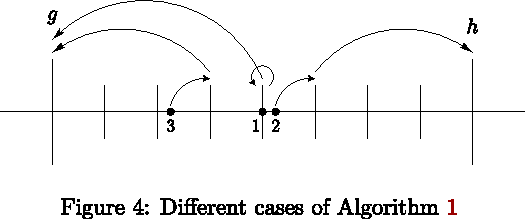
\includegraphics[width=0.8\textwidth]{assets/RR2004-48-Fig-4.pdf}
		\end{figure}

		--- Sylvie Boldo, Guillaume Melquiond.
		\href
		{https://hal-lara.archives-ouvertes.fr/hal-02101979/document}
		{When double rounding is odd}.
		[Research Report] LIP RR-2004-48, Laboratoire de l'informatique du parallélisme.
		2004, 2+7p.  hal-02101979
	\end{exampleblock}
\end{frame}

\subsection{Minifloats}
\begin{frame}{Minifloats}
	\begin{itemize}
		\item Minifloats are floating-point values represented with very few bits.
		\item Minifloats are usually special-purpose and tailored to their use cases.
		\item To save precious bit patterns, especially with its width within 8
		      bits, a minifloat format may
		      \begin{itemize}
			      \item Reserve fewer representations for infinities and NaNs.
			      \item Rebrand ``$-0$'' as NaN.
			      \item Use a non-default exponent bias for its use case.
		      \end{itemize}
	\end{itemize}
\end{frame}

\begin{frame}{Emulating minifloat operations}
	Consider emulating minifloat operations with native floating-point operations.

	\begin{itemize}
		\item Native operations are fast.
		\item Reusing conversion between minifloats and native floats improves
		      robustness by reducing code size.
		\item Such emulation is usually \textbf{bit-true}, assuming that the
		      rounding mode agrees in both types.  Native floats are usually at
		      least twice as wide as minifloats, which practically eliminates
		      the double rounding problem.
	\end{itemize}
\end{frame}

\begin{frame}{Common floating-point formats}
	Significand/mantissa grows faster than exponent.

	\begin{description}
		\item[binary64] E11M52
		\item[binary32] E8M23
		\item[binary16] E5M10
		\item[bfloat16] E8M7
		\item[float8] E\{\texttt{3\href{https://doc.rust-lang.org/std/ops/struct.RangeInclusive.html}{..=}5}\}M\{\texttt{2..=4}\}
	\end{description}
\end{frame}

\begin{frame}{Exhaustive bit-true verification}
	\begin{itemize}
		\item \href{https://core-math.gitlabpages.inria.fr/}{CORE-MATH} exhaustively tested univariate binary32 functions.
		\item It is feasible to iterate $2^{32}$ flops.
		\item It is feasible to exhaustively test a bivariate function taking at most 16 bits each.
	\end{itemize}
\end{frame}

\section{Transcendental functions}
\begin{frame}{Table maker's dilemma}
	\begin{itemize}
		\item Let $f =$ target transcendental function.
		\item Let $g =$ algebraic approximation of $f$.
		\item Let $\circ =$ rounding operation.
		\item We cannot prove $\circ f = \circ g$ a priori.
		\item Given any $f \left( x \right) \ne g \left( x \right)$, we cannot
		      be sure if a discontinuity of $\circ$ occurs in between!
	\end{itemize}
\end{frame}

\begin{frame}{\href{https://core-math.gitlabpages.inria.fr/}{CORE-MATH}}
	\begin{itemize}
		\item Correctly rounded in all \href{https://en.cppreference.com/w/c/numeric/fenv/FE_round}{C rounding modes}
		\item Univariate binary32 functions are exhaustively tested.
		\item The rest are tested with known hard-to-round cases.
	\end{itemize}
\end{frame}

\begin{frame}{\href{https://github.com/jdh8/metallic-rs}{\texttt{metallic}}}
	\begin{itemize}
		\item My correctly rounded math library in Rust (WIP)
		\item Correctly rounded in the default rounding mode
		      \begin{itemize}
			      \item Rounding half to even, the only rounding mode in most languages.
			      \item Directed rounding in C/C++ is only guaranteed if
			            \texttt{\#pragma STDC FENV\_ACCESS ON} is set.
		      \end{itemize}
		\item Usually faster than CORE-MATH
	\end{itemize}
\end{frame}

\end{document}